% !TeX root = q2.tex

\subsection{Stereo Rectification}

Refer to Figure \ref{fig:q2c-sr-process} for the process information (how different stages look).

\begin{figure}[ht]
    \centering
    \begin{subfigure}[b]{0.3 \textwidth}
        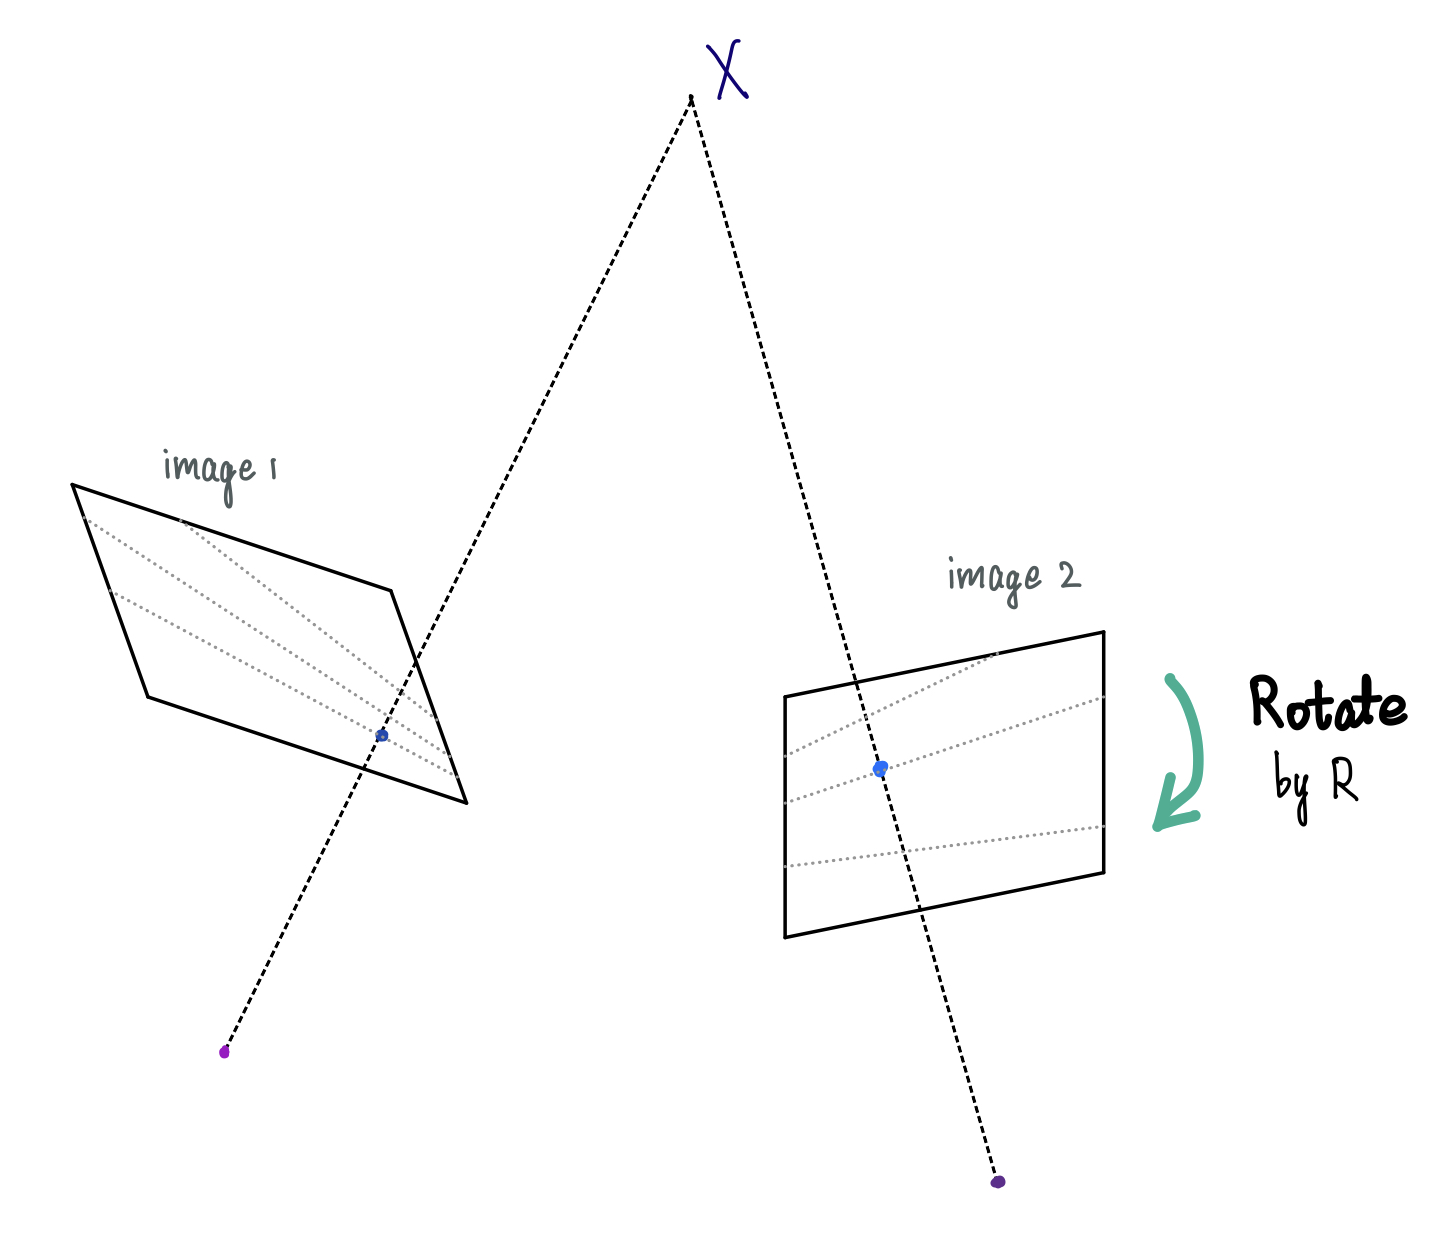
\includegraphics[width=\textwidth]{sr_s1.PNG}
        \caption{Stage 1}
        \label{fig:sfig-q2c-stage1}
    \end{subfigure}
    \begin{subfigure}[b]{0.3 \textwidth}
        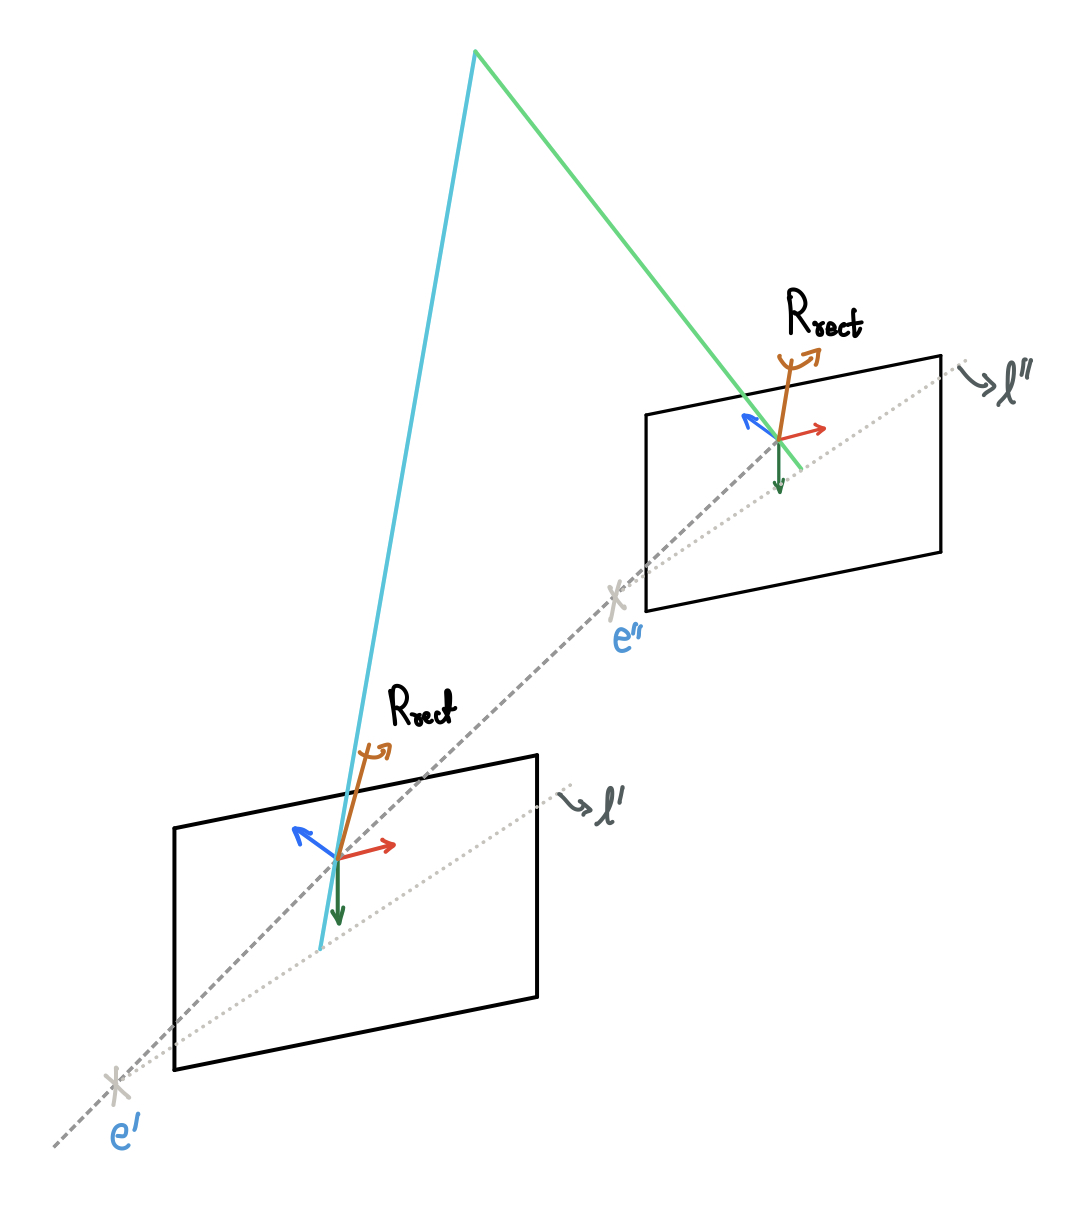
\includegraphics[width=\textwidth]{sr_s2.PNG}
        \caption{Stage 2}
        \label{fig:sfig-q2c-stage2}
    \end{subfigure}
    \begin{subfigure}[b]{0.3 \textwidth}
        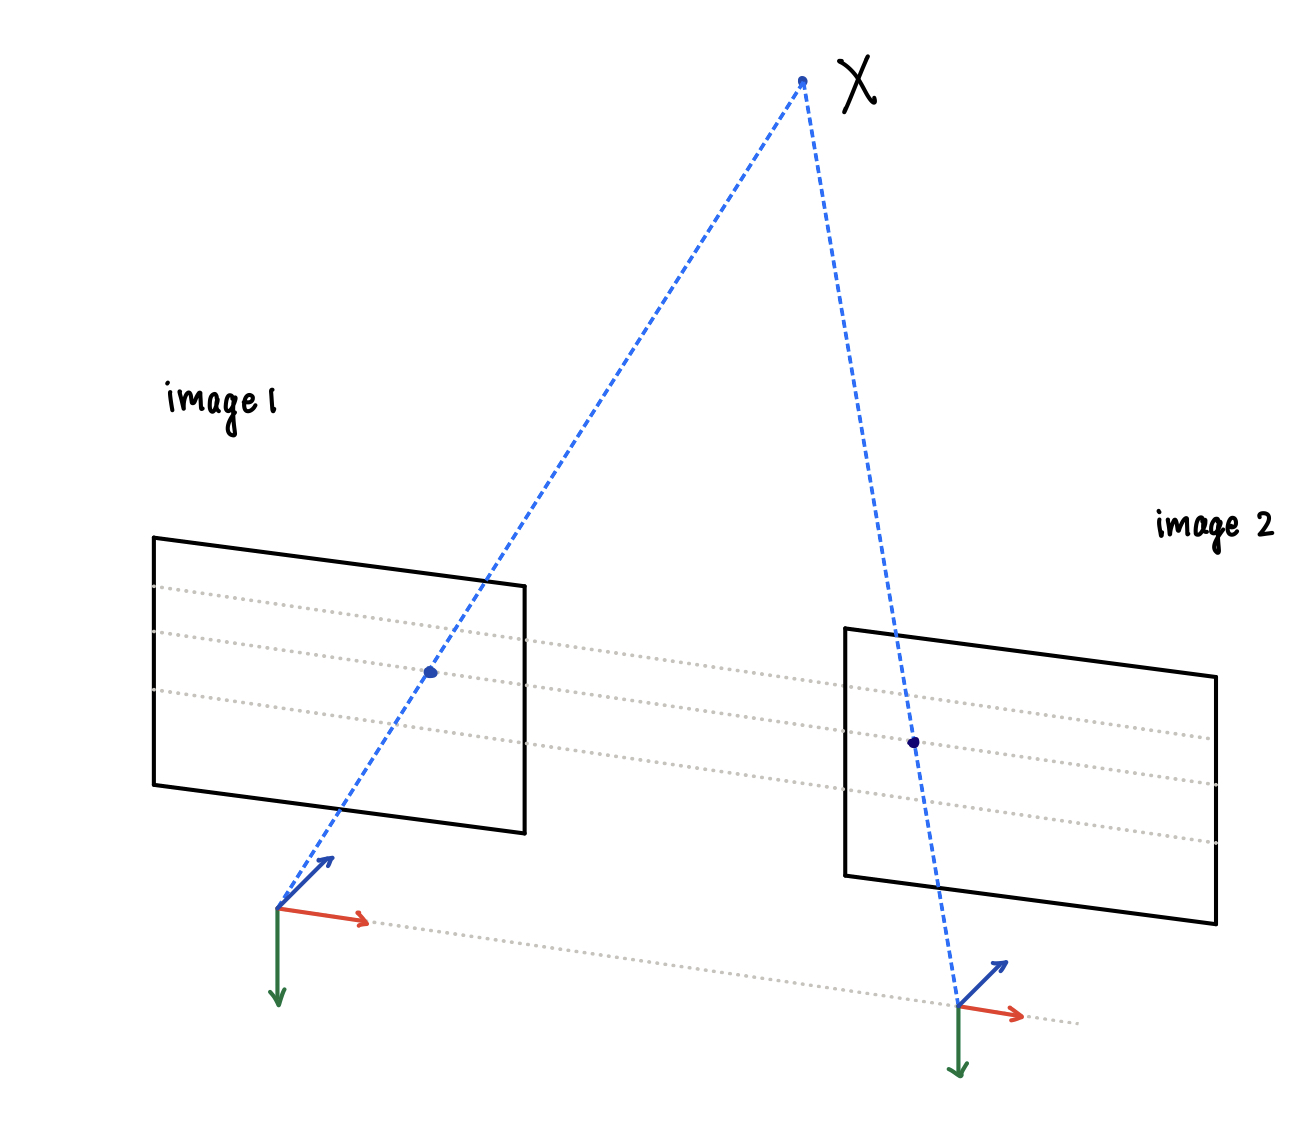
\includegraphics[width=\textwidth]{sr_s3.PNG}
        \caption{Stage 3}
        \label{fig:sfig-q2c-stage3}
    \end{subfigure}
    \caption{Stereo Rectification Process}
    \label{fig:q2c-sr-process}
    \small
        In the first stage (sub-fig. \ref{sub@fig:sfig-q2c-stage1}), the cameras have a rotation and a translation. Notice how the epipolar lines are arranged (grey dotted lines).
        
        A rotation (\textbf{first homography}) to the second image gives stage 2 (sub-fig. \ref{sub@fig:sfig-q2c-stage2}). Here, the images have no rotation (same orientation of cameras), but still there are (finite) epipoles, as shown by the grey line.
        
        Another rotation (\textbf{second homography}) has to be applied to both the images, so that they become co-planar and that the second camera's location is at the +X axis of the first. This way, all epipolar lines will become horizontal (as shown in sub-fig. \ref{sub@fig:sfig-q2c-stage3}).
\end{figure}

Before getting started, we need to calibrate the cameras (so that we know the intrinsics). After the calibration, we proceed with the following steps

\begin{enumerate}
    \item \textbf{First homography}: Here, we estimate the \textit{essential matrix} using 5 or 8 correspondences (depends on the 5-point or 8-point algorithm being used). Once we know $\mathbf{E}$, we represent the essential matrix as $\mathbf{E} = [\mathbf{b}]_\times \mathbf{R}^\top$. Here, we assume the first camera's frame as the reference. Using SVD of $\mathbf{E}$ (and resolving it into two parts), it is possible to get $\mathbf{R}$ (and the baseline translation vector $\mathbf{t} = \mathbf{b}$). Therefore, the first homography is to align the two images (align the second image with the first). The system changes from figure \ref{fig:sfig-q2c-stage1} to \ref{sub@fig:sfig-q2c-stage2}. Note from \ref{eq:q2a-rot-result} that the second image is transformed as $\mathbf{x}''_2 = \mathbf{KR} \mathbf{K}^{-1} \; \mathbf{x}''$.
    \item \textbf{Second homography}: From figure \ref{fig:sfig-q2c-stage2}, it is clear that even when the images are aligned, they needn't have poles at infinity. We need the poles at infinity and we also need the epipolar lines to be horizontal. Specifically, we need the epipoles at $\mathbf{e}' = [e'_x \; 0 \; 0]$ and $\mathbf{e}'' = [e''_x \; 0 \; 0]$ (in $\mathbb{P}^2$, in both the images), basically on the X axis at infinity.
    
    Note that epipoles are the null space of the fundamental matrix $\mathbf{F}$ (between the images). We need to construct a rotation matrix such that the new frames have only translational offset. Let's say that for stage 2, as shown in figure \ref{fig:sfig-q2c-stage2}, we get the epipoles as $\mathbf{e}' = [e'_x \; e'_y \; 1]$ (scaled to unit scaling factor). We resolve the rotation matrix $\mathbf{R}_{\textup{rect}}$ as

    \begin{align}
        \mathbf{r}_1 = \widehat{\mathbf{K}^{-1} \mathbf{e}''} = \frac{\overrightarrow{\mathbf{t}}}{\left \| \mathbf{t} \right \|}
        &&
        \mathbf{r}_2 = [0 \; 0 \; 1] \times \widehat{\mathbf{t}} = \frac{1}{\sqrt{t_x^2 + t_y^2}} \, [-t_y \; t_x \; 0]^\top
        &&
        \mathbf{r}_3 = \mathbf{r}_1 \times \mathbf{r}_2
    \end{align}

    Note that these are intuitively derived unit vectors to rotate the frame (of the left and right cameras) in figure \ref{sub@fig:sfig-q2c-stage2} to the frame (of the left and right cameras) in figure \ref{fig:sfig-q2c-stage3}. The final rotation matrix is

    \begin{equation}
        \mathbf{R}_{\textup{rect}} = \begin{bmatrix} \mathbf{r}_1^\top \\ \mathbf{r}_2^\top \\ \mathbf{r}_3^\top \end{bmatrix}
    \end{equation}

    Note that this homography of $\mathbf{H} = \mathbf{K} \, \mathbf{R}_{\textup{rect}} \, \mathbf{K}^{-1}$ has to be applied to both the images. This brings us from figure \ref{fig:sfig-q2c-stage2} to figure \ref{fig:sfig-q2c-stage3}.

    Finally, image one has become $\mathbf{x}'_3 = \mathbf{K} \, \mathbf{R}_{\textup{rect}} \, \mathbf{K}^{-1} \; \mathbf{x}'$.

    And image two has become $\mathbf{x}''_3 = \mathbf{K} \, \mathbf{R}_{\textup{rect}} \, \mathbf{K}^{-1} \; \mathbf{x}''_2$, which is the same as $\mathbf{x}''_3 = \mathbf{K} \, \mathbf{R}_{\textup{rect}} \, \mathbf{R} \, \mathbf{K}^{-1} \; \mathbf{x}''$.

    Also, note that since the basis vector was chosen as the $\mathbf{r}_1$, it will map the epipole to X axis (at infinity), other two $\mathbf{r}$ vectors will give zero as the dot product (they're by design perpendicular).

    \item There may be a scaling to get the pixels to the \textit{image pixel} representation (by scaling the last element in $\mathbb{P}^2$ vectors to 1).

\end{enumerate}

The first two steps above are called homographies because they largely deal with homogeneous coordinates (both as input and output) and also because they map points in one image directly to points in the other. This was also seen in equation \ref{eq:q2a-rot-result}.
